\section{Complete Results}
\label{app:full_results}

This appendix gives the full metric set for every condition of the main experimental blocks, as recorded by the aggregation pipeline of Section~\ref{subsec:metrics}. Each row is the mean over five seeds (three for the CIFAR generalisation block) with the seed standard deviation. Accuracy-type metrics (ACC, FORG, min-ACC, $\mathrm{WF}_{100}$, $\mathrm{WP}_{100}$, WC-ACC) are fractions; \texttt{gap\_depth} is in percentage points (pp); \texttt{gap\_area\_end} is the transient cost (accuracy-fraction $\times$ steps, Table~\ref{tab:gap_metrics}), the dip below the level each task recovers to, so permanent forgetting does not contribute; ``Recov.'' is \texttt{recovery\_steps}, with ``---'' marking conditions where every past task stayed above the $90\%$ recovery threshold for the whole window (no recovery event to time).

\subsection{rot-MNIST: Decomposition (D-series)}
\label{app:decomp_full}

\begin{table}[H]
    \centering
    \scriptsize
    \setlength{\tabcolsep}{4pt}
    \resizebox{\textwidth}{!}{%
        \begin{tabular}{l ccc cc c cc c}
            \hline
            Condition            & ACC                 & FORG                 & min-ACC             & $\mathrm{WF}_{100}$ & $\mathrm{WP}_{100}$ & WC-ACC              & Depth            & Area end        & Recov.           \\
            \hline
            \multicolumn{10}{l}{\emph{Momentum $0.0$}}                                                                                                                                                                        \\
            D1 vanilla           & 0.873\,$\pm$\,0.005 & 0.019\,$\pm$\,0.020  & 0.706\,$\pm$\,0.056 & 0.147\,$\pm$\,0.029 & 0.736\,$\pm$\,0.020 & 0.794\,$\pm$\,0.028 & 19.5\,$\pm$\,4.1 & 6.3\,$\pm$\,0.5 & 3.6\,$\pm$\,0.9  \\
            D2 fulldata          & 0.890\,$\pm$\,0.009 & -0.016\,$\pm$\,0.009 & 0.719\,$\pm$\,0.039 & 0.126\,$\pm$\,0.020 & 0.736\,$\pm$\,0.018 & 0.801\,$\pm$\,0.022 & 18.3\,$\pm$\,2.5 & 8.1\,$\pm$\,0.7 & 3.0\,$\pm$\,1.2  \\
            D3 balanced-dir      & 0.873\,$\pm$\,0.003 & 0.014\,$\pm$\,0.019  & 0.662\,$\pm$\,0.065 & 0.199\,$\pm$\,0.056 & 0.742\,$\pm$\,0.018 & 0.770\,$\pm$\,0.034 & 31.0\,$\pm$\,9.9 & 5.4\,$\pm$\,0.7 & 5.6\,$\pm$\,4.2  \\
            D4 fulldata bal-dir  & 0.894\,$\pm$\,0.003 & -0.036\,$\pm$\,0.014 & 0.675\,$\pm$\,0.061 & 0.190\,$\pm$\,0.065 & 0.738\,$\pm$\,0.016 & 0.772\,$\pm$\,0.030 & 31.4\,$\pm$\,13.7 & 3.0\,$\pm$\,1.3 & 6.2\,$\pm$\,6.1 \\
            M1 lr-warmup N50     & 0.846\,$\pm$\,0.026 & 0.045\,$\pm$\,0.024  & 0.666\,$\pm$\,0.047 & 0.170\,$\pm$\,0.034 & 0.743\,$\pm$\,0.004 & 0.762\,$\pm$\,0.026 & 21.5\,$\pm$\,5.2 & 5.7\,$\pm$\,0.5 & 44.4\,$\pm$\,5.5 \\
            M2 lr-warmup N100    & 0.839\,$\pm$\,0.025 & 0.050\,$\pm$\,0.024  & 0.706\,$\pm$\,0.032 & 0.153\,$\pm$\,0.027 & 0.726\,$\pm$\,0.005 & 0.777\,$\pm$\,0.024 & 17.5\,$\pm$\,3.7 & 4.9\,$\pm$\,0.5 & 76.4\,$\pm$\,9.9 \\
            M3 lr-warmup N200    & 0.815\,$\pm$\,0.025 & 0.068\,$\pm$\,0.030  & 0.738\,$\pm$\,0.009 & 0.111\,$\pm$\,0.013 & 0.698\,$\pm$\,0.004 & 0.777\,$\pm$\,0.015 & 14.3\,$\pm$\,1.4 & 2.7\,$\pm$\,0.4 & 125.0\,$\pm$\,6.9 \\
            \hline
            \multicolumn{10}{l}{\emph{Momentum $0.9$}}                                                                                                                                                                        \\
            D1 vanilla           & 0.928\,$\pm$\,0.003 & 0.058\,$\pm$\,0.007  & 0.797\,$\pm$\,0.028 & 0.092\,$\pm$\,0.016 & 0.808\,$\pm$\,0.012 & 0.878\,$\pm$\,0.014 & 15.9\,$\pm$\,2.6 & 1.0\,$\pm$\,0.2 & 12.6\,$\pm$\,1.7 \\
            D2 fulldata          & 0.964\,$\pm$\,0.002 & -0.010\,$\pm$\,0.003 & 0.807\,$\pm$\,0.009 & 0.082\,$\pm$\,0.004 & 0.808\,$\pm$\,0.012 & 0.885\,$\pm$\,0.004 & 14.9\,$\pm$\,0.9 & 3.1\,$\pm$\,0.2 & 10.6\,$\pm$\,1.1 \\
            D3 balanced-dir      & 0.933\,$\pm$\,0.004 & 0.037\,$\pm$\,0.004  & 0.830\,$\pm$\,0.029 & 0.078\,$\pm$\,0.012 & 0.808\,$\pm$\,0.011 & 0.889\,$\pm$\,0.013 & 12.6\,$\pm$\,2.8 & 1.6\,$\pm$\,0.5 & 8.0\,$\pm$\,5.5 \\
            D4 fulldata bal-dir  & 0.967\,$\pm$\,0.001 & -0.021\,$\pm$\,0.002 & 0.864\,$\pm$\,0.025 & 0.052\,$\pm$\,0.012 & 0.820\,$\pm$\,0.015 & 0.911\,$\pm$\,0.013 & 9.2\,$\pm$\,2.5  & 1.2\,$\pm$\,0.2 & 3.5\,$\pm$\,2.1  \\
            M1 lr-warmup N50     & 0.931\,$\pm$\,0.006 & 0.055\,$\pm$\,0.010  & 0.805\,$\pm$\,0.018 & 0.085\,$\pm$\,0.008 & 0.828\,$\pm$\,0.010 & 0.883\,$\pm$\,0.009 & 15.0\,$\pm$\,1.6 & 1.4\,$\pm$\,0.4 & 21.2\,$\pm$\,6.3 \\
            M2 lr-warmup N100    & 0.931\,$\pm$\,0.003 & 0.054\,$\pm$\,0.008  & 0.844\,$\pm$\,0.014 & 0.066\,$\pm$\,0.008 & 0.823\,$\pm$\,0.011 & 0.902\,$\pm$\,0.007 & 11.1\,$\pm$\,1.2 & 1.0\,$\pm$\,0.3 & 23.4\,$\pm$\,3.0 \\
            M3 lr-warmup N200    & 0.925\,$\pm$\,0.007 & 0.052\,$\pm$\,0.005  & 0.878\,$\pm$\,0.018 & 0.051\,$\pm$\,0.007 & 0.816\,$\pm$\,0.011 & 0.912\,$\pm$\,0.009 & 7.8\,$\pm$\,1.6  & 0.5\,$\pm$\,0.3 & 31.0            \\
            \hline
        \end{tabular}%
    }
    \caption{rot-MNIST step- and field-intervention block (revised D-series
        plus the M-series learning-rate warm-up), full metrics, at both
        momentum settings. For the balanced-direction conditions, depth reads
        the manufactured first step discussed in
        Section~\ref{subsec:res_levels}, not the excursion that follows.
        M3's momentum-$0.9$ recovery time is from the single seed with a
        recovery event. Buffer-fidelity diagnostics for these runs are in
        Table~\ref{tab:app_grad}. The original unit-norm balanced conditions
        are in Appendix~\ref{app:old_balanced}.}
    \label{tab:app_decomp}
\end{table}

\subsection{rot-MNIST: The Original Unit-Norm Balanced Conditions}
\label{app:old_balanced}

An earlier version of the driver block balanced the two gradients differently: each component was normalised to unit length, combined at equal weight, and the joint direction was then normalised to unit length again, so every update had length exactly $\eta$ regardless of the local gradient magnitude. These conditions (here labelled old D3 and old D4) appeared to remove the boundary spike outright, cutting depth from $19.5$ to $5.7$ pp on the sampled buffer and to $1.9$ pp on the exact one. The revised block shows where that reduction came from. At the boundary the raw joint gradient is at its largest, so fixing the step length at $\eta$ caps precisely the steps that produce the drop: the manipulation is a step-size intervention wearing a balancing costume. The balanced-direction conditions of the main text perform the same remix at vanilla's step length and deepen the drop instead (Figure~\ref{fig:old_balanced}), which is why the main text replaces these conditions rather than building on them. Full metrics below.

\begin{figure}[H]
    \centering
    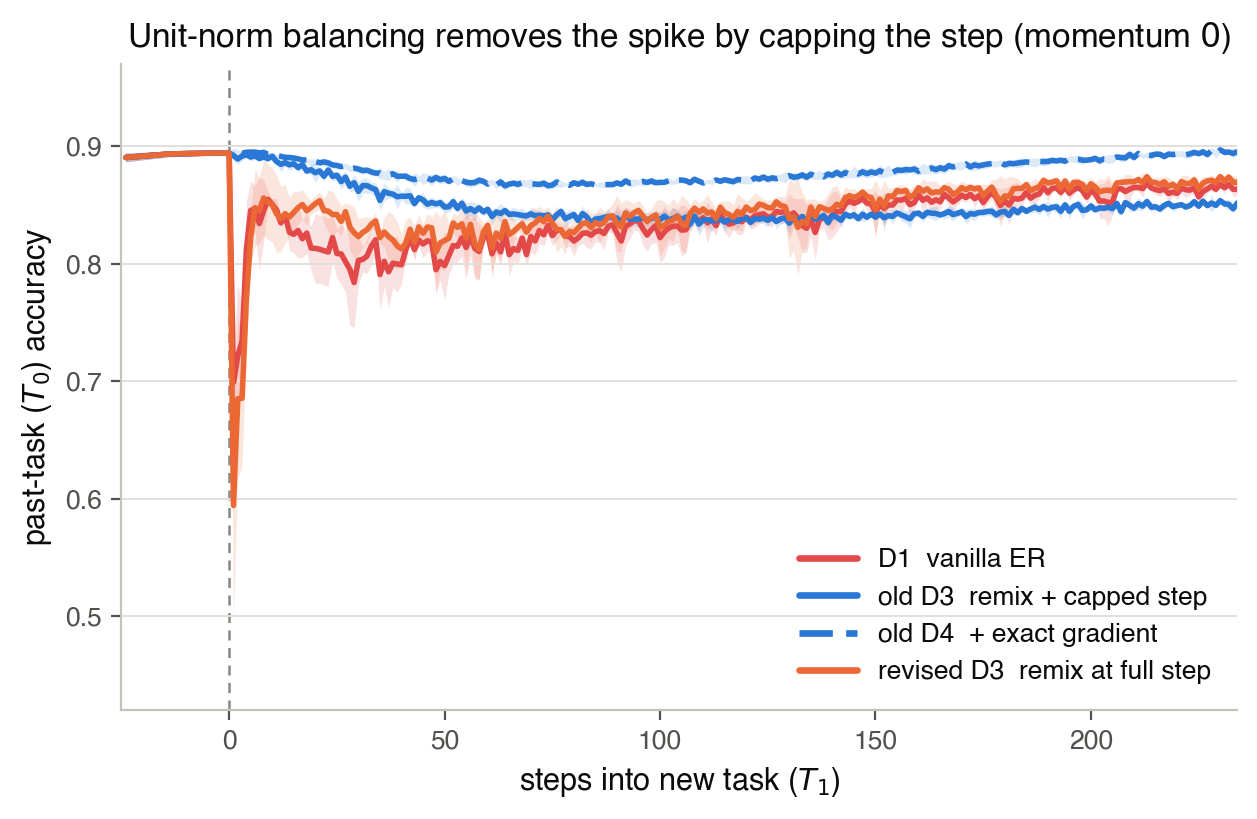
\includegraphics[width=0.72\linewidth]{img/results/D/old_balanced_t0.png}
    \caption{Per-step past-task ($T_0$) accuracy across the rot-MNIST switch at momentum $0$: vanilla ER (red), the original unit-norm balanced conditions (blue; dashed: exact gradient), and the revised balanced-direction condition at vanilla's step length (orange). The original conditions show no boundary spike because the unit normalisation caps the step exactly where the raw gradient is large; the same remix at full step length deepens the spike instead.}
    \label{fig:old_balanced}
\end{figure}

\begin{table}[H]
    \centering
    \scriptsize
    \setlength{\tabcolsep}{4pt}
    \resizebox{\textwidth}{!}{%
        \begin{tabular}{l ccc cc c cc c}
            \hline
            Condition            & ACC                 & FORG                 & min-ACC             & $\mathrm{WF}_{100}$ & $\mathrm{WP}_{100}$ & WC-ACC              & Depth            & Area end        & Recov.           \\
            \hline
            \multicolumn{10}{l}{\emph{Momentum $0.0$}}                                                                                                                                                                        \\
            old D3 unit-norm balanced & 0.849\,$\pm$\,0.005 & 0.031\,$\pm$\,0.018  & 0.824\,$\pm$\,0.006 & 0.045\,$\pm$\,0.002 & 0.721\,$\pm$\,0.004 & 0.836\,$\pm$\,0.004 & 5.7\,$\pm$\,1.9  & 1.4\,$\pm$\,0.4 & ---              \\
            old D4 fulldata unit-norm & 0.869\,$\pm$\,0.002 & -0.014\,$\pm$\,0.013 & 0.862\,$\pm$\,0.002 & 0.030\,$\pm$\,0.007 & 0.710\,$\pm$\,0.003 & 0.852\,$\pm$\,0.002 & 1.9\,$\pm$\,1.3  & 3.2\,$\pm$\,0.5 & ---              \\
            \hline
            \multicolumn{10}{l}{\emph{Momentum $0.9$}}                                                                                                                                                                        \\
            old D3 unit-norm balanced & 0.932\,$\pm$\,0.005 & 0.038\,$\pm$\,0.003  & 0.897\,$\pm$\,0.006 & 0.040\,$\pm$\,0.003 & 0.822\,$\pm$\,0.011 & 0.922\,$\pm$\,0.003 & 5.9\,$\pm$\,0.6  & 0.4\,$\pm$\,0.2 & ---              \\
            old D4 fulldata unit-norm & 0.967\,$\pm$\,0.001 & -0.022\,$\pm$\,0.003 & 0.942\,$\pm$\,0.005 & 0.016\,$\pm$\,0.004 & 0.834\,$\pm$\,0.010 & 0.950\,$\pm$\,0.002 & 1.3\,$\pm$\,0.4  & 0.2\,$\pm$\,0.1 & ---              \\
            \hline
        \end{tabular}%
    }
    \caption{The original unit-norm balanced conditions, full metrics. The
        low depths are produced by the step cap, not by the remix; see the
        text of this appendix and Section~\ref{subsec:res_levels}.}
    \label{tab:app_old_balanced}
\end{table}

\subsection{rot-MNIST: \texorpdfstring{$\lambda$}{lambda}-Curriculum (C-series)}
\label{app:curr_full}

\begin{table}[H]
    \centering
    \scriptsize
    \setlength{\tabcolsep}{4pt}
    \resizebox{\textwidth}{!}{%
        \begin{tabular}{l ccc cc c cc c}
            \hline
            Condition            & ACC                 & FORG                & min-ACC             & $\mathrm{WF}_{100}$ & $\mathrm{WP}_{100}$ & WC-ACC              & Depth            & Area end        & Recov.             \\
            \hline
            \multicolumn{10}{l}{\emph{Momentum $0.0$}}                                                                                                                                                                         \\
            C1 linear N50        & 0.851\,$\pm$\,0.023 & 0.042\,$\pm$\,0.021 & 0.707\,$\pm$\,0.019 & 0.148\,$\pm$\,0.011 & 0.748\,$\pm$\,0.006 & 0.784\,$\pm$\,0.021 & 17.5\,$\pm$\,1.7 & 4.9\,$\pm$\,0.5 & 35.8\,$\pm$\,6.3   \\
            C2 linear N100       & 0.844\,$\pm$\,0.025 & 0.046\,$\pm$\,0.023 & 0.719\,$\pm$\,0.033 & 0.140\,$\pm$\,0.025 & 0.730\,$\pm$\,0.006 & 0.786\,$\pm$\,0.019 & 16.2\,$\pm$\,4.3 & 3.6\,$\pm$\,0.3 & 64.0\,$\pm$\,8.6   \\
            C3 linear N200       & 0.828\,$\pm$\,0.025 & 0.054\,$\pm$\,0.024 & 0.739\,$\pm$\,0.048 & 0.128\,$\pm$\,0.043 & 0.688\,$\pm$\,0.004 & 0.784\,$\pm$\,0.034 & 14.3\,$\pm$\,4.6 & 1.8\,$\pm$\,0.6 & 132.8\,$\pm$\,43.4 \\
            C4 adaptive          & 0.833\,$\pm$\,0.025 & 0.050\,$\pm$\,0.019 & 0.754\,$\pm$\,0.025 & 0.111\,$\pm$\,0.016 & 0.703\,$\pm$\,0.007 & 0.794\,$\pm$\,0.020 & 12.8\,$\pm$\,2.9 & 2.2\,$\pm$\,0.5 & 88.8\,$\pm$\,6.1   \\
            C5 adaptive lmin0.05 & 0.835\,$\pm$\,0.025 & 0.048\,$\pm$\,0.019 & 0.749\,$\pm$\,0.027 & 0.113\,$\pm$\,0.016 & 0.702\,$\pm$\,0.006 & 0.793\,$\pm$\,0.020 & 13.2\,$\pm$\,3.2 & 2.2\,$\pm$\,0.5 & 88.8\,$\pm$\,6.1   \\
            C6 adaptive lmin0.10 & 0.836\,$\pm$\,0.026 & 0.048\,$\pm$\,0.021 & 0.743\,$\pm$\,0.026 & 0.120\,$\pm$\,0.019 & 0.700\,$\pm$\,0.007 & 0.791\,$\pm$\,0.019 & 13.9\,$\pm$\,3.3 & 2.4\,$\pm$\,0.5 & 88.4\,$\pm$\,11.0  \\
            C7 adaptive lmin0.20 & 0.837\,$\pm$\,0.031 & 0.049\,$\pm$\,0.024 & 0.743\,$\pm$\,0.030 & 0.119\,$\pm$\,0.023 & 0.710\,$\pm$\,0.010 & 0.792\,$\pm$\,0.024 & 13.9\,$\pm$\,3.4 & 2.7\,$\pm$\,0.6 & 64.8\,$\pm$\,8.2   \\
            \hline
            \multicolumn{10}{l}{\emph{Momentum $0.9$}}                                                                                                                                                                         \\
            C1 linear N50        & 0.932\,$\pm$\,0.003 & 0.053\,$\pm$\,0.005 & 0.892\,$\pm$\,0.004 & 0.041\,$\pm$\,0.004 & 0.830\,$\pm$\,0.012 & 0.927\,$\pm$\,0.003 & 6.4\,$\pm$\,0.5  & 0.2\,$\pm$\,0.1 & ---                \\
            C2 linear N100       & 0.932\,$\pm$\,0.003 & 0.051\,$\pm$\,0.008 & 0.892\,$\pm$\,0.005 & 0.036\,$\pm$\,0.003 & 0.826\,$\pm$\,0.012 & 0.926\,$\pm$\,0.002 & 6.4\,$\pm$\,0.6  & 0.2\,$\pm$\,0.1 & ---                \\
            C3 linear N200       & 0.925\,$\pm$\,0.007 & 0.051\,$\pm$\,0.006 & 0.893\,$\pm$\,0.004 & 0.031\,$\pm$\,0.004 & 0.819\,$\pm$\,0.010 & 0.920\,$\pm$\,0.006 & 6.2\,$\pm$\,0.6  & 0.1\,$\pm$\,0.0 & ---                \\
            C4 adaptive          & 0.917\,$\pm$\,0.001 & 0.019\,$\pm$\,0.004 & 0.931\,$\pm$\,0.005 & 0.016\,$\pm$\,0.003 & 0.798\,$\pm$\,0.010 & 0.915\,$\pm$\,0.001 & 2.5\,$\pm$\,0.5  & 0.3\,$\pm$\,0.1 & ---                \\
            C5 adaptive lmin0.05 & 0.922\,$\pm$\,0.001 & 0.023\,$\pm$\,0.004 & 0.930\,$\pm$\,0.005 & 0.016\,$\pm$\,0.002 & 0.802\,$\pm$\,0.009 & 0.921\,$\pm$\,0.001 & 2.6\,$\pm$\,0.5  & 0.1\,$\pm$\,0.0 & ---                \\
            C6 adaptive lmin0.10 & 0.927\,$\pm$\,0.002 & 0.028\,$\pm$\,0.005 & 0.926\,$\pm$\,0.004 & 0.017\,$\pm$\,0.003 & 0.806\,$\pm$\,0.009 & 0.927\,$\pm$\,0.002 & 3.0\,$\pm$\,0.4  & 0.0\,$\pm$\,0.0 & ---                \\
            C7 adaptive lmin0.20 & 0.931\,$\pm$\,0.002 & 0.035\,$\pm$\,0.005 & 0.919\,$\pm$\,0.003 & 0.021\,$\pm$\,0.004 & 0.812\,$\pm$\,0.009 & 0.930\,$\pm$\,0.001 & 3.7\,$\pm$\,0.4  & 0.0\,$\pm$\,0.0 & ---                \\
            \hline
        \end{tabular}%
    }
    \caption{rot-MNIST $\lambda$-curriculum sweep, full metrics, at both momentum
        settings. All conditions applied on top of standard ER (1\,k reservoir).}
    \label{tab:app_curr}
\end{table}

\paragraph{Full-buffer momentum diagnostic (C8).}
Table~\ref{tab:res_c8} crosses the practical curriculum with the full $60$k buffer
at both momentum settings, isolating momentum's two roles (Section~\ref{subsec:res_scalar}).
Source variance reduction alone (C8, full buffer, $\mu{=}0$) already closes the
gap to $0.2$ pp, so the residual the curriculum leaves at $\mu{=}0$ is estimator
variance, not structure; momentum's gap-closing role is interchangeable with the
full buffer. Acceleration alone (the $\mu{=}0.9$ column) restores accuracy: C8$_M$
reaches $0.955$, approaching the full-data ceiling (D2$_M$: $0.964$), while
re-introducing a small transient ($2.0$ pp, area $0.38$). The shape and timing
of this transient point to the $\lambda_{\min}$ floor meeting momentum. With
the replay gradient exact and the arc removed, the only push left in the first
steps is the floored fifth of the new-task gradient (the logged gradient-norm
ratio confirms the schedule sits at $\lambda = 0.2$ through the dip window),
and momentum amplifies a persistent push toward $1/(1-\mu) = 10$ times its
per-step size: the dip accordingly opens at the boundary, bottoms out about
ten steps in, and closes within about fifty as the replay gradient reasserts
itself. The floor is by construction the one share of the push the source gate
does not attenuate, so momentum briefly re-inflates exactly that share, a
miniature of the directional gate's re-inflation. The dose-response on the
same exact buffer supports the reading: the floored push without momentum
costs $0.2$ pp (C8), with momentum $2.0$ pp (C8$_M$), and the unfloored
abrupt switch with momentum $14.9$ pp (D2$_M$). C8$_M$'s area additionally
counts in full under the end-referencing convention of
Section~\ref{subsec:metrics}, since it recovers above its pre-switch level. C8/C8$_M$ are diagnostic probes: the full buffer defeats the limited-memory
premise, and the practical scalar-gate configuration remains C7$_M$
($3.7$ pp / $0.03$ / $0.931$) at $1/60$th the memory.

\begin{table}[H]
    \centering
    \small
    \begin{tabular}{l cccc}
        \hline
                                 & C7              & C7$_M$            & C8                & C8$_M$              \\
                                 & (1k, $\mu{=}0$) & (1k, $\mu{=}0.9$) & (full, $\mu{=}0$) & (full, $\mu{=}0.9$) \\
        \hline
        \texttt{gap\_depth} (pp) & $13.9$          & $3.7$             & $\mathbf{0.2}$    & $2.0$               \\
        \texttt{gap\_area\_end}  & $2.7$           & $0.03$            & $\mathbf{0.05}$   & $0.38$              \\
        ACC                      & $0.837$         & $0.931$           & $0.818$           & $\mathbf{0.955}$    \\
        \hline
    \end{tabular}
    \caption{Curriculum $\times$ full buffer $\times$ momentum on rot-MNIST,
        isolating momentum's two roles. Source variance reduction alone (C8) closes
        the gap; acceleration alone (the $\mu$ column) restores accuracy. The residual
        at C7 ($\mu{=}0$) is variance, not structure.}
    \label{tab:res_c8}
\end{table}

\subsection{rot-MNIST: Buffer-Fidelity Diagnostics}
\label{app:grad_full}

The gradient diagnostics of Appendix~\ref{subsubsec:grad_metrics} were logged for
the decomposition block only. The full-data conditions (D2, D4) reach exact
fidelity by construction, the replay gradient equals the deterministic
empirical past-task gradient, so cosine and magnitude ratio are $1.000$. The
finite-buffer conditions (D1, D3) show the directional and magnitude error a
$1{,}000$-sample reservoir incurs against $g_{\text{true}}$.

\begin{table}[H]
    \centering
    \scriptsize
    \setlength{\tabcolsep}{4pt}
    \begin{tabular}{l ccc}
        \hline
        Condition                 & $\bar{\cos}$        & $\cos_{\min}$        & $\bar{\rho}$        \\
        \hline
        D1 vanilla ($\mu{=}0$)    & 0.711\,$\pm$\,0.035 & 0.086\,$\pm$\,0.103  & 1.040\,$\pm$\,0.039 \\
        D3 balanced ($\mu{=}0$)   & 0.665\,$\pm$\,0.043 & 0.025\,$\pm$\,0.140  & 1.137\,$\pm$\,0.060 \\
        D1 vanilla ($\mu{=}0.9$)  & 0.551\,$\pm$\,0.033 & 0.135\,$\pm$\,0.069  & 0.418\,$\pm$\,0.014 \\
        D3 balanced ($\mu{=}0.9$) & 0.441\,$\pm$\,0.039 & -0.052\,$\pm$\,0.117 & 0.265\,$\pm$\,0.024 \\
        D2, D4 (full data)        & 1.000               & 1.000                & 1.000               \\
        \hline
    \end{tabular}
    \caption{Buffer-fidelity diagnostics for the decomposition block:
        $\bar{\cos}$ and $\cos_{\min}$ are the mean and minimum of
        $\cos(g_{\text{replay}}, g_{\text{true}})$ over the window; $\bar{\rho}$ is the
        mean of $\|g_{\text{replay}}\|/\|g_{\text{true}}\|$.}
    \label{tab:app_grad}
\end{table}

\subsection{rot-MNIST: Asymmetric PER (P-series)}
\label{app:per_full}

Table~\ref{tab:app_per_full} gives the full metric set for the asymmetric-PER
$\delta$ sweep on both buffer legs and at both momentum settings; the momentum-$0$
depth/area/ACC columns match Table~\ref{tab:res_per} in the main text, and the
momentum-$0.9$ rows are the source of the re-inflation numbers of
Section~\ref{subsec:res_directional}. Momentum-$0.9$ runs cover the three
strongest filters on the standard leg and $\delta \in \{0.3, 0.1\}$ on the
full-buffer leg.

\begin{table}[H]
    \centering
    \scriptsize
    \setlength{\tabcolsep}{4pt}
    \resizebox{\textwidth}{!}{%
        \begin{tabular}{l ccc cc c cc}
            \hline
            Condition                 & ACC                 & FORG                 & min-ACC             & $\mathrm{WF}_{100}$ & $\mathrm{WP}_{100}$ & WC-ACC              & Depth             & Area end          \\
            \hline
            \multicolumn{9}{l}{\emph{Standard ($1$k) buffer, momentum $0.0$}}                                                                                                                                      \\
            $\delta{=}1.0$            & 0.869\,$\pm$\,0.005 & 0.027\,$\pm$\,0.018  & 0.792\,$\pm$\,0.012 & 0.081\,$\pm$\,0.009 & 0.733\,$\pm$\,0.009 & 0.838\,$\pm$\,0.006 & 9.0\,$\pm$\,0.6   & 3.29\,$\pm$\,0.65 \\
            $\delta{=}0.3$            & 0.873\,$\pm$\,0.004 & 0.023\,$\pm$\,0.017  & 0.807\,$\pm$\,0.012 & 0.068\,$\pm$\,0.009 & 0.736\,$\pm$\,0.008 & 0.847\,$\pm$\,0.005 & 7.4\,$\pm$\,1.1   & 2.32\,$\pm$\,0.59 \\
            $\delta{=}0.1$            & 0.876\,$\pm$\,0.004 & 0.018\,$\pm$\,0.016  & 0.822\,$\pm$\,0.012 & 0.056\,$\pm$\,0.009 & 0.739\,$\pm$\,0.008 & 0.856\,$\pm$\,0.005 & 5.9\,$\pm$\,1.5   & 1.56\,$\pm$\,0.65 \\
            $\delta{=}0.03$           & 0.880\,$\pm$\,0.005 & 0.012\,$\pm$\,0.015  & 0.834\,$\pm$\,0.012 & 0.048\,$\pm$\,0.005 & 0.741\,$\pm$\,0.007 & 0.862\,$\pm$\,0.005 & 4.8\,$\pm$\,1.9   & 1.04\,$\pm$\,0.58 \\
            \multicolumn{9}{l}{\emph{Standard ($1$k) buffer, momentum $0.9$}}                                                                                                                                      \\
            $\delta{=}0.3$            & 0.929\,$\pm$\,0.002 & 0.061\,$\pm$\,0.004  & 0.851\,$\pm$\,0.008 & 0.065\,$\pm$\,0.004 & 0.813\,$\pm$\,0.009 & 0.907\,$\pm$\,0.005 & 10.4\,$\pm$\,0.5  & 0.50\,$\pm$\,0.17 \\
            $\delta{=}0.1$            & 0.928\,$\pm$\,0.002 & 0.061\,$\pm$\,0.006  & 0.861\,$\pm$\,0.008 & 0.060\,$\pm$\,0.005 & 0.815\,$\pm$\,0.009 & 0.911\,$\pm$\,0.005 & 9.4\,$\pm$\,0.5   & 0.38\,$\pm$\,0.19 \\
            $\delta{=}0.03$           & 0.929\,$\pm$\,0.003 & 0.060\,$\pm$\,0.009  & 0.871\,$\pm$\,0.008 & 0.053\,$\pm$\,0.007 & 0.816\,$\pm$\,0.010 & 0.917\,$\pm$\,0.005 & 8.5\,$\pm$\,0.6   & 0.23\,$\pm$\,0.12 \\
            \hline
            \multicolumn{9}{l}{\emph{Full ($60$k) buffer, momentum $0.0$}}                                                                                                                                         \\
            $\delta{=}1.0$            & 0.898\,$\pm$\,0.002 & -0.025\,$\pm$\,0.012 & 0.841\,$\pm$\,0.011 & 0.037\,$\pm$\,0.011 & 0.734\,$\pm$\,0.006 & 0.865\,$\pm$\,0.006 & 4.0\,$\pm$\,1.0   & 2.32\,$\pm$\,1.38 \\
            $\delta{=}0.3$            & 0.900\,$\pm$\,0.002 & -0.029\,$\pm$\,0.012 & 0.867\,$\pm$\,0.002 & 0.026\,$\pm$\,0.007 & 0.739\,$\pm$\,0.005 & 0.878\,$\pm$\,0.002 & 1.5\,$\pm$\,1.1   & 1.01\,$\pm$\,0.91 \\
            $\delta{=}0.1$            & 0.901\,$\pm$\,0.002 & -0.032\,$\pm$\,0.013 & 0.860\,$\pm$\,0.026 & 0.040\,$\pm$\,0.028 & 0.741\,$\pm$\,0.004 & 0.875\,$\pm$\,0.013 & 2.2\,$\pm$\,1.6   & 0.44\,$\pm$\,0.38 \\
            $\delta{=}0.03$           & 0.903\,$\pm$\,0.002 & -0.035\,$\pm$\,0.012 & 0.787\,$\pm$\,0.094 & 0.118\,$\pm$\,0.102 & 0.742\,$\pm$\,0.004 & 0.838\,$\pm$\,0.048 & 9.5\,$\pm$\,8.2   & 0.43\,$\pm$\,0.25 \\
            $\delta{=}0.03$ (CG $60$) & 0.903\,$\pm$\,0.002 & -0.035\,$\pm$\,0.012 & 0.766\,$\pm$\,0.113 & 0.126\,$\pm$\,0.109 & 0.742\,$\pm$\,0.004 & 0.828\,$\pm$\,0.057 & 11.5\,$\pm$\,10.1 & 0.47\,$\pm$\,0.28 \\
            \multicolumn{9}{l}{\emph{Full ($60$k) buffer, momentum $0.9$}}                                                                                                                                         \\
            $\delta{=}0.3$            & 0.964\,$\pm$\,0.001 & -0.012\,$\pm$\,0.002 & 0.864\,$\pm$\,0.009 & 0.052\,$\pm$\,0.005 & 0.813\,$\pm$\,0.008 & 0.913\,$\pm$\,0.005 & 9.1\,$\pm$\,0.8   & 1.91\,$\pm$\,0.26 \\
            $\delta{=}0.1$            & 0.965\,$\pm$\,0.001 & -0.012\,$\pm$\,0.003 & 0.880\,$\pm$\,0.008 & 0.044\,$\pm$\,0.004 & 0.814\,$\pm$\,0.008 & 0.921\,$\pm$\,0.005 & 7.6\,$\pm$\,0.7   & 1.57\,$\pm$\,0.25 \\
            \hline
        \end{tabular}%
    }
    \caption{rot-MNIST asymmetric-PER $\delta$ sweep, full metrics: both buffer
        legs at both momentum settings, plus the solver control (CG $60$). The
        momentum-$0.9$ rows show the re-inflation of
        Section~\ref{subsec:res_directional}: depth climbs on every leg relative to
        its momentum-$0$ counterpart, while the full-buffer accuracies
        (${\approx}0.965$) are diagnostic values only, the full buffer defeating the limited-memory premise.}
    \label{tab:app_per_full}
\end{table}

\subsection{rot-MNIST: Symmetric vs.\ Asymmetric Preconditioning}
\label{app:per_sym}

Leaving the restoring gradient $g_{\text{rep}}$ at full strength is the directional
gate's defining choice (Section~\ref{subsec:res_directional}). The alternative is to
precondition the summed update, $d = \delta(F_{\text{rep}}+\delta I)^{-1}(g_{\text{cur}}+g_{\text{rep}})$,
the symmetric variant that passes both gradients through the same metric. Because
$g_{\text{rep}}$ is the gradient of the replay loss, it lies in the top eigenspace of that
loss's own Fisher $F_{\text{rep}}$, so the symmetric filter shrinks the restoring
gradient \emph{harder} than the harmful push it is meant to brake and cannot
preferentially protect the past task. Table~\ref{tab:res_per_sym} sweeps the same
$\delta$ on both variants, and they are mirror images. As the filter strengthens
($\delta \to 0$) the asymmetric gate's forgetting falls (FORG $0.027 \to 0.012$) and its
accuracy rises, while the symmetric gate's forgetting \emph{climbs} ($0.030 \to 0.066$)
and its accuracy falls; every one of these four trends holds across all five seeds.
Symmetric depth barely moves across the sweep ($5.7 \to 6.7$ pp) and at $\delta{=}1.0$
even sits below the asymmetric gate's ($5.7$ vs.\ $9.0$ pp), because filtering the whole
update also damps the per-step \emph{expression} of the dip. This is the area caveat of
Section~\ref{subsec:metrics} made concrete: the symmetric gate's end-referenced area
collapses toward zero ($2.7 \to 0.01$) not because the dip recovers but because it stops
recovering, settling into a permanent accommodation that the area excludes and the
forgetting metric records. Read on depth or transient area the symmetric gate looks
competitive; read on forgetting and final accuracy it degrades monotonically as its
filter strengthens. Asymmetry is what turns the filter from a reshuffling of the damage
into a net removal of it.

\begin{table}[H]
    \centering
    \small
    \begin{tabular}{l cccc c cccc}
        \hline
                 & \multicolumn{4}{c}{Asymmetric ($g_{\text{rep}}$ free)} &           & \multicolumn{4}{c}{Symmetric (joint)}                                                              \\
        \cline{2-5}\cline{7-10}
        $\delta$ & depth (pp)                                             & area      & FORG                                  & ACC     &  & depth (pp) & area   & FORG    & ACC     \\
        \hline
        $1.0$    & $9.0$                                                  & $3.29$    & $0.027$                               & $0.869$ &  & $5.7$      & $2.69$ & $0.030$ & $0.872$ \\
        $0.3$    & $7.4$                                                  & $2.32$    & $0.023$                               & $0.873$ &  & $5.9$      & $1.65$ & $0.042$ & $0.867$ \\
        $0.1$    & $5.9$                                                  & $1.56$    & $0.018$                               & $0.876$ &  & $6.2$      & $0.34$ & $0.057$ & $0.861$ \\
        $0.03$   & $4.8$                                                  & $1.04$    & $0.012$                               & $0.880$ &  & $6.7$      & $0.01$ & $0.066$ & $0.857$ \\
        \hline
    \end{tabular}
    \caption{Asymmetric versus symmetric preconditioning on the standard $1$k buffer at
        momentum $0$, five seeds, sweeping the shared damping $\delta$. Both variants filter
        through the replay Fisher $F_{\text{rep}}$; they differ only in whether the metric is
        applied to the new-task push alone (asymmetric, $g_{\text{rep}}$ left free) or to the
        summed update (symmetric). As $\delta \to 0$ the asymmetric gate improves on every
        axis while the symmetric gate degrades on every axis; symmetric depth stays flat
        because the filter suppresses the per-step expression of the dip even as the
        underlying forgetting grows, and the symmetric end-referenced area collapses
        toward zero for the same reason: the past task stops recovering, so the loss
        registers in FORG rather than in the transient area (Section~\ref{subsec:metrics}).}
    \label{tab:res_per_sym}
\end{table}

\subsection{CIFAR-10: Headline Block}
\label{app:cifar_headline_full}

\begin{table}[H]
    \centering
    \scriptsize
    \setlength{\tabcolsep}{4pt}
    \resizebox{\textwidth}{!}{%
        \begin{tabular}{l ccc cc c cc}
            \hline
            Condition        & ACC                 & FORG                 & min-ACC             & $\mathrm{WF}_{100}$ & $\mathrm{WP}_{100}$ & WC-ACC              & Depth             & Area end          \\
            \hline
            G1 vanilla BN    & 0.723\,$\pm$\,0.008 & 0.010\,$\pm$\,0.019  & 0.644\,$\pm$\,0.023 & 0.127\,$\pm$\,0.015 & 0.484\,$\pm$\,0.020 & 0.667\,$\pm$\,0.016 & 11.8\,$\pm$\,2.5  & 17.5\,$\pm$\,4.6  \\
            G2 adaptive BN   & 0.722\,$\pm$\,0.011 & 0.006\,$\pm$\,0.016  & 0.713\,$\pm$\,0.017 & 0.070\,$\pm$\,0.010 & 0.469\,$\pm$\,0.016 & 0.698\,$\pm$\,0.013 & 4.8\,$\pm$\,0.7   & 3.6\,$\pm$\,2.2   \\
            G3 asym.\ PER BN & 0.715\,$\pm$\,0.011 & -0.008\,$\pm$\,0.018 & 0.698\,$\pm$\,0.023 & 0.124\,$\pm$\,0.022 & 0.460\,$\pm$\,0.025 & 0.682\,$\pm$\,0.023 & 5.9\,$\pm$\,4.3   & 3.3\,$\pm$\,3.0   \\
            G4 vanilla GN    & 0.730\,$\pm$\,0.011 & -0.023\,$\pm$\,0.030 & 0.309\,$\pm$\,0.111 & 0.294\,$\pm$\,0.097 & 0.415\,$\pm$\,0.058 & 0.507\,$\pm$\,0.054 & 41.2\,$\pm$\,13.5 & 34.9\,$\pm$\,23.7 \\
            G5 adaptive GN   & 0.731\,$\pm$\,0.020 & -0.026\,$\pm$\,0.026 & 0.670\,$\pm$\,0.055 & 0.095\,$\pm$\,0.033 & 0.340\,$\pm$\,0.052 & 0.687\,$\pm$\,0.037 & 5.2\,$\pm$\,2.1   & 1.7\,$\pm$\,0.9   \\
            G6 asym.\ PER GN & 0.741\,$\pm$\,0.009 & -0.035\,$\pm$\,0.018 & 0.673\,$\pm$\,0.023 & 0.080\,$\pm$\,0.009 & 0.330\,$\pm$\,0.024 & 0.696\,$\pm$\,0.015 & 5.6\,$\pm$\,1.1   & 4.8\,$\pm$\,3.8   \\
            \hline
        \end{tabular}%
    }
    \caption{CIFAR-10 headline block, full metrics (ResNet-18, momentum $0.9$,
        buffer $5{,}000$, five seeds). ``adaptive'' is the practical curriculum with
        $\lambda_{\min} = 0.20$; ``asym.\ PER'' runs at $\delta = 0.1$.}
    \label{tab:app_cifar_headline}
\end{table}

\paragraph{The gates' residual batch-norm dip.}
The small gap the gates keep under batch norm is a genuine boundary transient:
in Figure~\ref{fig:cifar_curves}(a) both gated curves dip together over the
first steps after the switch, by roughly the tabulated $5$ pp, and recover to
their plateau within a few tens of steps. A reading consistent with this
pattern is the normalisation pathway of Section~\ref{subsec:cifar}. BatchNorm's
running statistics update on every forward pass, whatever the gate does to the
gradient, so the first corrupted batches shift them away from the clean task
and no gate on the update can hold that back; the clean replay samples in every
batch pull the statistics back, which matches the fast recovery. The group-norm
contrast supports the reading: with no cross-batch statistics to disturb, the
curriculum holds $T_0$ flat through the same boundary
(Figure~\ref{fig:cifar_curves}(b)) and its transient area falls to roughly half
its batch-norm value ($1.7$ vs.\ $3.6$). This is a reading rather than an
established mechanism; a control that freezes the running statistics across
the switch would isolate it.

\subsection{CIFAR-10: Generalisation Block}
\label{app:cifar_gen_full}

Each shift pairs the practical curriculum (``curric.'': adaptive $\lambda_{\min} =
    0.20$, buffer $5{,}000$) against a vanilla-ER control on the same shift, at the
indicated normalisation, over three seeds.

\begin{table}[H]
    \centering
    \scriptsize
    \setlength{\tabcolsep}{4pt}
    \begin{tabular}{l ccc c cc}
        \hline
        Condition              & ACC                 & FORG                 & min-ACC             & WC-ACC              & Depth             & Area end          \\
        \hline
        \multicolumn{7}{l}{\emph{BatchNorm}}                                                                                                                    \\
        shot noise (vanilla) & 0.724\,$\pm$\,0.011 & 0.017\,$\pm$\,0.010  & 0.633\,$\pm$\,0.017 & 0.663\,$\pm$\,0.014 & 13.1\,$\pm$\,3.0  & 21.2\,$\pm$\,3.9  \\
        shot noise (curric.) & 0.723\,$\pm$\,0.014 & 0.010\,$\pm$\,0.010  & 0.708\,$\pm$\,0.032 & 0.697\,$\pm$\,0.016 & 5.6\,$\pm$\,1.0   & 5.8\,$\pm$\,1.5   \\
        contrast (vanilla)   & 0.671\,$\pm$\,0.026 & -0.008\,$\pm$\,0.006 & 0.610\,$\pm$\,0.063 & 0.586\,$\pm$\,0.048 & 15.4\,$\pm$\,3.9  & 33.4\,$\pm$\,4.5  \\
        contrast (curric.)   & 0.671\,$\pm$\,0.044 & -0.012\,$\pm$\,0.007 & 0.727\,$\pm$\,0.034 & 0.643\,$\pm$\,0.048 & 3.7\,$\pm$\,1.1   & 2.2\,$\pm$\,0.9   \\
        3-task (vanilla)     & 0.740\,$\pm$\,0.006 & -0.011\,$\pm$\,0.013 & 0.670\,$\pm$\,0.015 & 0.691\,$\pm$\,0.010 & 3.3\,$\pm$\,0.4   & 6.0\,$\pm$\,0.7   \\
        3-task (curric.)     & 0.745\,$\pm$\,0.010 & -0.021\,$\pm$\,0.008 & 0.677\,$\pm$\,0.025 & 0.696\,$\pm$\,0.017 & 6.9\,$\pm$\,2.7   & 3.9\,$\pm$\,0.1   \\
        \hline
        \multicolumn{7}{l}{\emph{GroupNorm}}                                                                                                                    \\
        shot noise (vanilla) & 0.718\,$\pm$\,0.021 & -0.036\,$\pm$\,0.036 & 0.244\,$\pm$\,0.075 & 0.469\,$\pm$\,0.032 & 46.3\,$\pm$\,12.0 & 54.4\,$\pm$\,40.8 \\
        shot noise (curric.) & 0.705\,$\pm$\,0.061 & -0.028\,$\pm$\,0.012 & 0.638\,$\pm$\,0.108 & 0.656\,$\pm$\,0.087 & 7.3\,$\pm$\,5.9   & 2.4\,$\pm$\,1.1   \\
        contrast (vanilla)   & 0.777\,$\pm$\,0.022 & -0.067\,$\pm$\,0.021 & 0.641\,$\pm$\,0.061 & 0.710\,$\pm$\,0.040 & 8.4\,$\pm$\,4.4   & 3.3\,$\pm$\,0.6   \\
        contrast (curric.)   & 0.778\,$\pm$\,0.032 & -0.070\,$\pm$\,0.013 & 0.668\,$\pm$\,0.077 & 0.724\,$\pm$\,0.054 & 3.9\,$\pm$\,3.1   & 1.2\,$\pm$\,0.8   \\
        3-task (vanilla)     & 0.722\,$\pm$\,0.020 & -0.023\,$\pm$\,0.015 & 0.468\,$\pm$\,0.043 & 0.550\,$\pm$\,0.023 & 4.4\,$\pm$\,0.4   & 10.3\,$\pm$\,3.6  \\
        3-task (curric.)     & 0.721\,$\pm$\,0.019 & -0.025\,$\pm$\,0.020 & 0.421\,$\pm$\,0.114 & 0.517\,$\pm$\,0.070 & 32.8\,$\pm$\,14.5 & 32.0\,$\pm$\,19.5 \\
        \hline
    \end{tabular}
    \caption{CIFAR-10 generalisation block, full metrics. The two-task novel
        corruptions (shot noise, contrast) favour the curriculum under both
        normalisations; the three-task group-norm sequence is the outlier analysed
        below.}
    \label{tab:app_cifar_gen}
\end{table}

\paragraph{The three-task group-norm failure.}
The three-task sequence is the one place the curriculum underperforms its
control (depth $32.8 \pm 14.5$ pp against vanilla's $4.4 \pm 0.4$,
Table~\ref{tab:app_cifar_gen}; Figure~\ref{fig:failure_curves}), and the logged
gradient-norm traces locate the failure in the conditioning of the feedback
signal. The adaptive ratio $r = \|g_{\text{replay}}\|/\|g_{\text{new}}\|$
carries information through the boundary ordering of
Section~\ref{subsec:curriculum}: at a well-separated switch the new-task
gradient dwarfs the replay gradient, so $r$ starts near zero and its rise
tracks the replay gradient reasserting itself. The first boundary of this
sequence behaves that way (clean $\rightarrow$ Gaussian: first-step new-task
loss $1.9$--$2.1$, $r \approx 0.2$), and the schedule holds every past task
flat through it. The second boundary never establishes the ordering: Gaussian
and shot noise are near-identical, so the incoming model already fits the new
task ($T_2$ accuracy $0.67$--$0.71$ before its first step, new-task loss
$0.5$--$0.7$), leaving $\|g_{\text{new}}\|$ small, while
$\|g_{\text{replay}}\|$ is small because the model is converged on the
replayed tasks. The ratio becomes a quotient of two near-zero norms: under
group norm it reads $0.5$--$1.3$ from the first step and fluctuates step to
step, so the EMA drives $\lambda$ from the floor to ${\approx}0.7$--$0.8$
within fifty steps and back to $\lambda_{\min}$ within a few hundred. The gate
is moved by noise, not by damage.

What follows, in all three seeds, is not a stability gap but an optimisation
instability. Within the first forty steps the replay loss itself diverges
($0.2$--$0.4 \rightarrow 0.8$--$2.1$) and every task falls together,
\emph{including the one being trained} ($T_2$: $0.71 \rightarrow 0.29$,
$0.69 \rightarrow 0.30$, $0.67 \rightarrow 0.51$ across seeds), before the run
recovers; the per-seed depth scales with the divergence, which is where the
$\pm 14.5$ pp spread comes from. Because all tasks crash together, the depth
and area of the three-task group-norm rows record this instability, not the
past-task transient the rest of the study measures. Two controls isolate the
trigger. The vanilla run crosses the same boundary with a flat replay loss and
$4.4$ pp of depth, so the near-identical boundary is harmless on its own; the
batch-norm run executes the identical schedule through the same boundary, with
the same ill-conditioned early ratio, without instability
(Figure~\ref{fig:failure_curves}), so the noise-driven $\lambda$ is not
sufficient either. The failure needs both the unconditioned signal and the
group-norm backbone's boundary sensitivity, consistent with the far deeper
group-norm transients vanilla ER shows on the same corruption family (shot
noise: $46.3$ vs $13.1$ pp, Table~\ref{tab:app_cifar_gen}). We therefore read
the episode as a reliability boundary of the gradient-norm-ratio signal rather
than of the gate principle: the ratio loses its meaning when both norms become
small, and the design admits direct guards: freezing $\lambda$ when both
norms fall below a reference scale, or reading a damage signal that does not
vanish at a quiet boundary, such as the replay-loss excess over its pre-switch
level.

\begin{figure}[H]
    \centering
    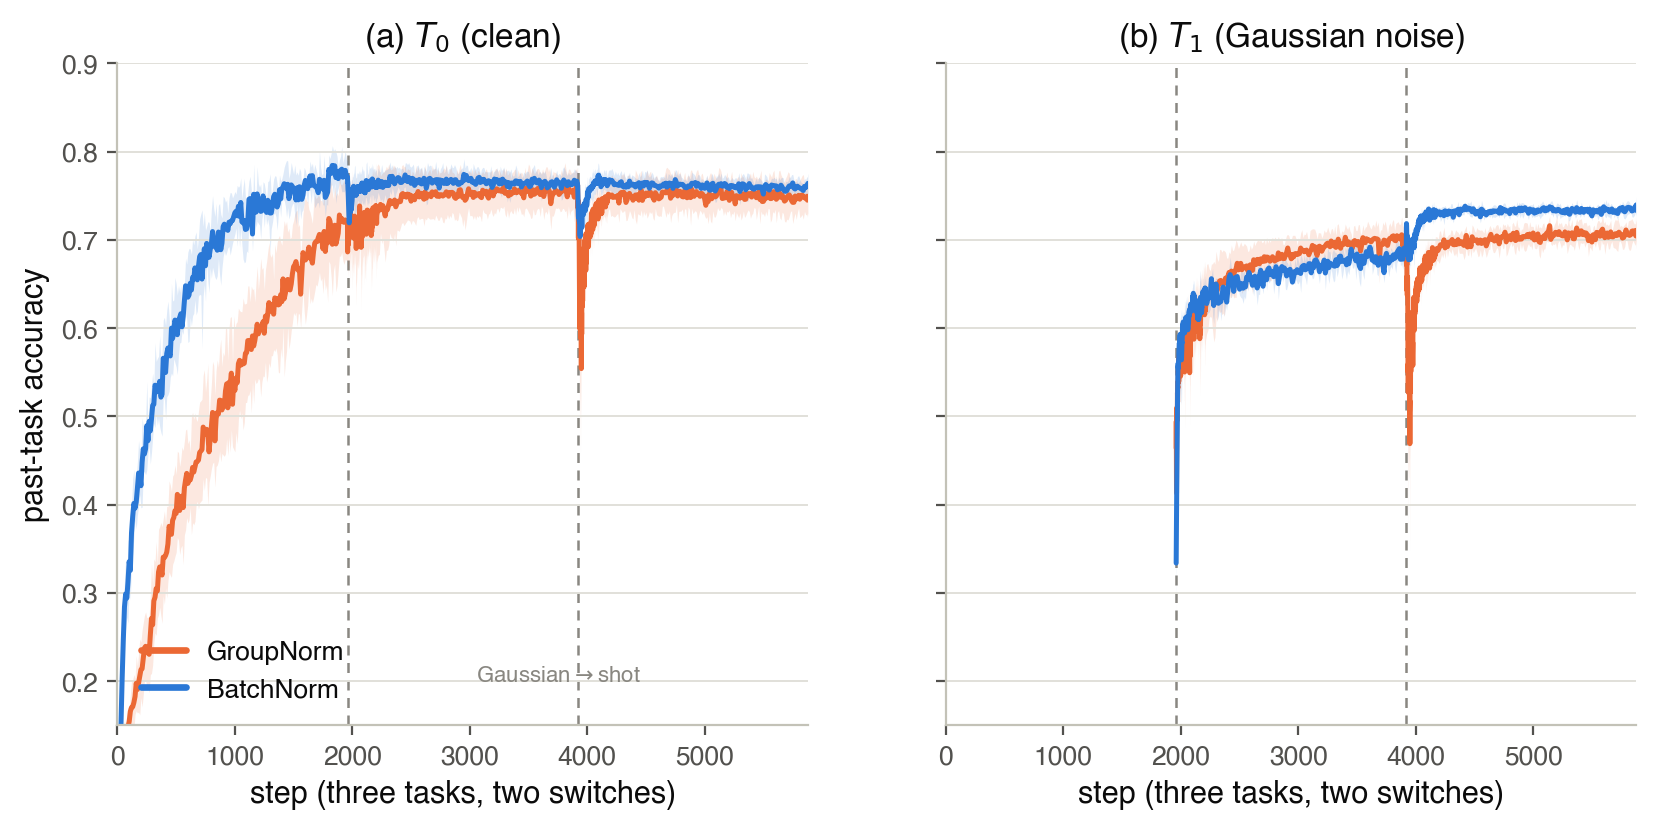
\includegraphics[width=\linewidth]{img/results/T/cifar_3task_failure.png}
    \caption{Per-step past-task accuracy across the three-task CIFAR-10
        generalisation sequence (none $\rightarrow$ Gaussian $\rightarrow$ shot,
        ResNet-18, practical curriculum, three seeds with $\pm$std bands), comparing
        the group-norm run (orange) against its batch-norm counterpart (blue). The
        two switches (dashed) fall at ${\sim}2$k and ${\sim}4$k steps. The first
        boundary (none $\rightarrow$ Gaussian) barely perturbs the past tasks in
        either norm. The second (Gaussian $\rightarrow$ shot, two near-identical
        corruptions) drives a deep transient in $T_0$ (a) and $T_1$ (b) under group
        norm only, while the batch-norm run holds flat through both switches. The dip
        is thus localised entirely to the second transition and to group norm, the
        adaptive-ratio reliability boundary analysed above.}
    \label{fig:failure_curves}
\end{figure}

\subsection{CIFAR-10: Momentum Cross and Compute Cost}
\label{app:cifar_extra}

This subsection collects the three deep-backbone checks summarised in
Section~\ref{subsec:res_cifar}: the momentum cross (Table~\ref{tab:res_cifar_mom}),
the generalisation block (Table~\ref{tab:app_cifar_gen} above), and the compute cost
(Table~\ref{tab:res_cost}).

\paragraph{Momentum cross.}
The cross repeats the composability test of Section~\ref{subsec:momentum} on the
ResNet, pairing momentum-$0$ runs at group norm against the momentum-$0.9$ rows,
and it turns out to be only weakly informative. At momentum $0$ the ResNet
under-converges the past task in ten epochs (vanilla min-ACC $0.11$, ACC $0.65$), so
every momentum-$0$ depth sits on a degraded baseline. On that baseline both gates
improve with momentum by similar margins (curriculum $28.6 \rightarrow 5.2$ pp,
asymmetric PER $22.6 \rightarrow 5.6$ pp), so the cross cannot separate the predicted
source-attenuation composition from a general convergence gain, and the prediction
that momentum re-inflates the directional gate does not appear; the vanilla null
($40.5 \rightarrow 41.2$ pp) is directionally consistent with the account but rests
on the same degraded baseline. We therefore draw no mechanism conclusion from this
cross in either direction: the momentum signatures rest on the rot-MNIST results,
where the MLP isolates them cleanly (Sections~\ref{subsec:res_scalar}
and~\ref{subsec:res_directional}), and a clean deep-backbone test would need a
converged momentum-$0$ baseline (Section~\ref{subsec:disc_limits}).

\begin{table}[H]
    \centering
    \small
    \begin{tabular}{l cc}
        \hline
        Method (GroupNorm)                   & depth, $\mu{=}0$ & depth, $\mu{=}0.9$ \\
        \hline
        Vanilla ER                           & $40.5 \pm 4.0$   & $41.2 \pm 13.5$    \\
        Curriculum ($\lambda_{\min}{=}0.20$) & $28.6 \pm 8.8$   & $5.2 \pm 2.1$      \\
        Asym.\ PER ($\delta{=}0.1$)          & $22.6 \pm 9.7$   & $5.6 \pm 1.1$      \\
        \hline
    \end{tabular}
    \caption{CIFAR-10 momentum cross (group norm, buffer $5{,}000$, five seeds), gap
        depth in pp. All momentum-$0$ cells sit on an under-converged baseline
        (vanilla min-ACC $0.11$), so the cross is read as uninformative for the
        momentum signatures rather than as partial confirmation (see text).}
    \label{tab:res_cifar_mom}
\end{table}

\paragraph{Compute cost.}
Cost is measured with a dedicated benchmark: one full two-task run per gate in its
headline configuration (curriculum: adaptive schedule, $\lambda_{\min}{=}0.20$;
asymmetric PER: $\delta{=}0.1$, $25$ warm-started CG iterations; momentum $0.9$,
group norm and buffer $5{,}000$ on CIFAR), five seeds each on a single NVIDIA RTX
PRO~6000, with per-step stability evaluation disabled so the numbers reflect method
compute alone. Wall-clock and CPU time come from \texttt{getrusage}; GPU utilisation,
power, and memory are sampled at $1$\,Hz with \texttt{nvidia-smi}, and energy is the
integrated power. On the ResNet-18 the split is stark (Table~\ref{tab:res_cost}). The
scalar gate adds one gradient-norm ratio and an EMA update to a standard ER step, and
its run is not even compute-bound: the GPU sits half-idle at $49\%$ utilisation and
$259$\,W. The directional gate's $25$ conjugate-gradient Fisher-vector products per
step, each on the order of a backward pass, saturate the same card ($96\%$, $367$\,W)
for $16\times$ as long, and since energy is power times time the two factors compound
to a $24\times$ energy gap ($13$ vs.\ $320$\,Wh per run). Memory is not the price:
peak GPU memory differs by $11\%$. On the rot-MNIST MLP both gates finish in under
half a minute at near-idle utilisation (the wall-clock is fixed startup, not method
compute), so no meaningful ratio exists there and the cost question is decided
entirely on the deep backbone. The ratios are the transferable claim; the absolute
numbers are specific to this card, and because ${\sim}15$--$30$\,s of each run is
startup, the training-only ratio is if anything slightly above $16\times$.

\begin{table}[H]
    \centering
    \small
    \begin{tabular}{ll ccccc}
        \hline
        Dataset & Gate & wall [s] & util [\%] & power [W] & energy [Wh] & mem [MB] \\
        \hline
        CIFAR-10 & Curriculum (scalar)         & $198 \pm 7$      & $49$    & $259$ & $13$  & $4{,}203$ \\
        (ResNet-18) & Asym.\ PER ($\delta{=}0.1$) & $3{,}157 \pm 11$ & $96$    & $367$ & $320$ & $4{,}679$ \\
        \hline
        rot-MNIST & Curriculum (scalar)         & $25 \pm 1$       & $<\!1$  & ---   & $0.4$ & $749$     \\
        (MLP) & Asym.\ PER ($\delta{=}0.1$) & $29 \pm 1$       & $8$     & ---   & $0.5$ & $769$     \\
        \hline
    \end{tabular}
    \caption{Compute cost of one full two-task run (mean over five seeds, $\pm$ sd on
        wall-clock; single RTX PRO 6000; per-step evaluation disabled): wall-clock, mean
        GPU utilisation and power, integrated GPU energy, and peak GPU memory. On the
        ResNet-18 the directional gate costs ${\sim}16\times$ the wall-clock and
        ${\sim}24\times$ the energy of the scalar gate at similar peak memory. The MLP
        rows are dominated by fixed startup on a near-idle GPU, so their power draw is
        idle draw (omitted) and no ratio is meaningful.}
    \label{tab:res_cost}
\end{table}

\subsection{Long-Sequence rot-MNIST (L-series)}
\label{app:longseq_full}

\begin{table}[H]
    \centering
    \scriptsize
    \setlength{\tabcolsep}{4pt}
    \resizebox{\textwidth}{!}{%
        \begin{tabular}{l ccc cc c cc}
            \hline
            Condition                             & ACC                 & FORG                & min-ACC             & $\mathrm{WF}_{100}$ & $\mathrm{WP}_{100}$ & WC-ACC              & Depth            & Area end          \\
            \hline
            \multicolumn{9}{l}{\emph{Momentum $0.0$}}                                                                                                                                                                        \\
            L1 vanilla ER                         & 0.861\,$\pm$\,0.004 & 0.060\,$\pm$\,0.004 & 0.670\,$\pm$\,0.055 & 0.207\,$\pm$\,0.053 & 0.443\,$\pm$\,0.011 & 0.722\,$\pm$\,0.043 & 21.0\,$\pm$\,5.8 & 3.14\,$\pm$\,0.77 \\
            L2 curriculum $\lambda_{\min}{=}0.20$ & 0.860\,$\pm$\,0.002 & 0.031\,$\pm$\,0.005 & 0.828\,$\pm$\,0.007 & 0.073\,$\pm$\,0.005 & 0.400\,$\pm$\,0.003 & 0.840\,$\pm$\,0.005 & 4.1\,$\pm$\,0.8  & 1.62\,$\pm$\,0.42 \\
            L3 asym.\ PER $\delta{=}0.1$          & 0.870\,$\pm$\,0.003 & 0.053\,$\pm$\,0.006 & 0.843\,$\pm$\,0.008 & 0.038\,$\pm$\,0.007 & 0.381\,$\pm$\,0.003 & 0.862\,$\pm$\,0.007 & 4.7\,$\pm$\,1.2  & 0.38\,$\pm$\,0.24 \\
            \hline
            \multicolumn{9}{l}{\emph{Momentum $0.9$}}                                                                                                                                                                        \\
            L1 vanilla ER                         & 0.889\,$\pm$\,0.007 & 0.096\,$\pm$\,0.008 & 0.845\,$\pm$\,0.007 & 0.065\,$\pm$\,0.008 & 0.317\,$\pm$\,0.006 & 0.870\,$\pm$\,0.006 & 8.9\,$\pm$\,1.7  & 1.68\,$\pm$\,0.69 \\
            L2 curriculum $\lambda_{\min}{=}0.20$ & 0.897\,$\pm$\,0.002 & 0.071\,$\pm$\,0.003 & 0.871\,$\pm$\,0.005 & 0.041\,$\pm$\,0.004 & 0.364\,$\pm$\,0.005 & 0.888\,$\pm$\,0.004 & 5.4\,$\pm$\,0.6  & 0.60\,$\pm$\,0.14 \\
            L3 asym.\ PER $\delta{=}0.1$          & 0.884\,$\pm$\,0.004 & 0.104\,$\pm$\,0.004 & 0.849\,$\pm$\,0.006 & 0.054\,$\pm$\,0.004 & 0.325\,$\pm$\,0.005 & 0.873\,$\pm$\,0.005 & 7.5\,$\pm$\,1.5  & 0.80\,$\pm$\,0.63 \\
            \hline
        \end{tabular}%
    }
    \caption{Five-task rot-MNIST (rotations $[0,30,60,90,120]^\circ$, four
        consecutive transitions, five seeds), the L-series: both gates in their
        practical configurations against vanilla ER, at both momentum settings.
        Depth is the worst single-boundary drop and area the end-referenced
        transient, aggregated as in the two-task blocks. At momentum $0$ both gates
        cut the depth from $21$ pp to ${\approx}4$ pp; under momentum the curriculum
        keeps the best cumulative retention while the re-inflated directional gate
        falls slightly behind vanilla on FORG ($0.104$ vs.\ $0.096$, all five seeds).}
    \label{tab:app_longseq}
\end{table}

\begin{figure}[H]
    \centering
    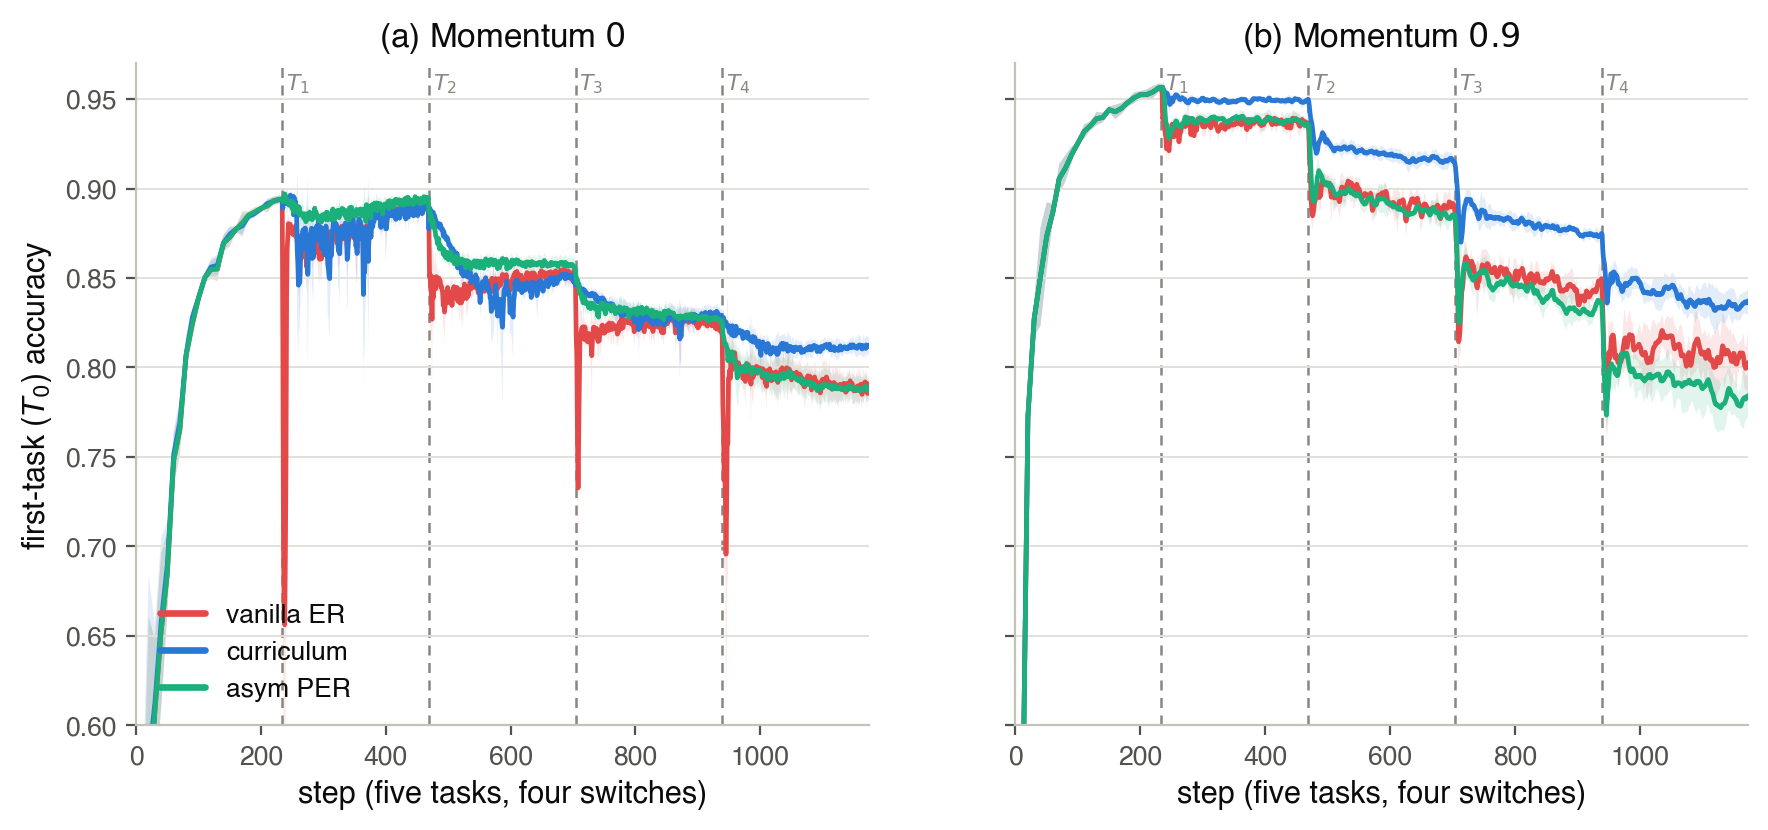
\includegraphics[width=\linewidth]{img/results/L/longseq.png}
    \caption{Five-task rot-MNIST (rotations $[0,30,60,90,120]^\circ$, four
        consecutive switches, five seeds with $\pm$std bands), the
        L-series: first-task $T_0$ accuracy across the whole sequence for vanilla ER
        (red), the practical curriculum $\lambda_{\min}{=}0.20$ (blue) and asymmetric
        PER $\delta{=}0.1$ (aqua); dashed lines mark the four switches, and the two
        panels are the two momentum settings. \textbf{(a) Momentum $0$:} both gates
        hold $T_0$ almost flat through every boundary, asymmetric PER the smoothest,
        while vanilla ER drops sharply at each switch. \textbf{(b) Momentum $0.9$:}
        PER's boundary transients return as momentum re-inflates its per-step filter
        (Section~\ref{subsec:res_directional}); the curriculum keeps the boundaries
        smoothest and holds the highest plateau (Table~\ref{tab:app_longseq}).}
    \label{fig:longseq}
\end{figure}

